\documentclass[letterpaper]{article}
\usepackage{natbib,alifexi}
\usepackage[utf8]{inputenc}
\usepackage[english]{babel}
\usepackage[colorinlistoftodos,prependcaption,textsize=tiny]{todonotes}


\title{Reinforcement learning approaches to movies recommendation}
\author{Antoine Carpentier$^{1}$, Pierre Gérard$^{2}$ \and Julian Schembri$^2$ \\
\mbox{}\\
$^1$Vrije Universiteit Brussel, Brussels \\
$^2$Université libre de Bruxelles, Brussels \\
antoine.carpentier@vub.ac.be, pierre.gerard@ulb.ac.be, julian.schembri@ulb.ac.be}


\begin{document}
\maketitle

\begin{abstract}
  The purpose of this research is to study a reinforcement learning approaches to building a cold-start recommender system. The reinforcement learning task formulate the problem of interactive recommendation as learning user preferences while doing an exploration-exploitation trade-off thus allowing us to provide to the user novelty content. This paper explore a content based learning as well as collaborative filtering learning, both yielding viable recommendation results.
\end{abstract}

\section{Introduction}


People sometimes have to settle on decisions without sufficient individual experience of the choices. In regular daily existence, we depend on  recommendations from other individuals either by listening in conversations or by direct suggestion of movies, tv show, holiday destination, etc. Recommender systems help and enlarge this normal social process. 

In a recommender system, individuals usually give behaviour information as data sources, which the system then use to learn users preferences in order to provide recommendation. The recommender's value lies in its capacity to make great matches between the recommenders and those looking for suggestions. Such systems are the strength of content providers such Netflix \cite{netflix-article-recommender} or YouTube \footnote{http://www.youtube.com} allowing them to make their content more attractive in order to increase viewing and in order to optimise its monetisation. It allows to infer customer's center of interest and also allows to detect, if a behaviour is a general trend between customers, potential improvements in content to better meet the expectations of the public. 


This work follows the steps of \cite{main} who have implemented a music recommendation system using q-learning. In their research, \cite{main} explains was could be done to adapt their work to movies recommendation as well as a suggestion trying a collaborative filtering. So this work, is mainly about adapting their strategy of music recommendation to movies recommendation as well as exploring new strategies.

The problem of movie recommendation is modelised as a multi-armed bandit [\cite{sutton1998reinforcement}] thus allowing it to have the following advantages. 

\begin{itemize}
	\item The learning is done by incorporating user feedback (i.e. ratings of movies) into recommendations allowing us to fit diversity in users preferences,
	\item The model takes into account novelty of movies and repetitions thus not recommending movies watched recently,
	\item The learngin balances exploration and exploitation thus mitigating the difficulty of cold-start,
	\item The model can take into account both a content based approaches and a collaborative filtering approaches.
\end{itemize}


In the following sections, we will firstly introduce methods used. Then we will review different results before discussing them.

\section{Methods}

\subsection{Data mining}

The data used is originated from IMDb \footnote{http://www.imdb.com/}. It is twofolds, the first part is a movie catalog containing relevant information about each movies such as the genre, keywords describing the content, the year, the rating by others users and votes count. That part is publicly available from IMDb FTP in a homemade format. The second part of data is RSS flux of movies watched and rated by IMDb users containing the title of the movie along the rating and the time it was watched.

\subsection{Features extraction and selection}

The first challenges was to extract the feature from the IMDb homemade format and made into a clearer \textit{csv} format.

In order to reduce the complexity of the algorithm and focus on the learning matter and not transforming the problem into a big data and parallelisation problem problem, a subset of movie, a selection of user and movies adding up to about 430.000 user-movie pair have been made.

Then for each movie and to also keep the problem simple and focus on the learning matter, we selected genre and year as features for each movie. Those two features are categorical variable and in order to learn a single weight per feature (i.e. drama, crime, ..), a onehot encoding have been apply to them resulting in a blow up of the feature space to $n$ features, $n$ being the number of category.

\begin{table}[h]
\center{
\begin{tabular}{|c|c|c|c|c|}\hline
 Name       & Drama & Crime & Thriller & ... \\ \hline
Movie 1  & 0   & 0 & 1 & ...\\ \hline
Movie 2  & 1 & 1 & 1 & ...\\ \hline
Movie 3  & 0 &   0 & 0 & ...\\ \hline
... & ... & ... &  ... \\ \hline
\end{tabular}
}
\vskip 0.25cm
\caption{Movise feature space}
\end{table}


\todo{ les fetaures selectionne et encodage onehot et pourquoi}
Then most of the feature were categorical variable


\subsection{Dimension reduction}

\todo{ comment et pouquoi on a fait une reduction de dimension}
In order to 


\subsection{Multi armed bandit modelisation}

\todo{comment on a modelise le probelem en bandit}

\subsection{Selections algorithms}

\todo{description des approches utilisés}


\subsection{Content based or collaborative filtering}

\todo{expliquer ces deux approches}


\section{Results}


\section{Discussion}


\section{Acknowledgements}

blabla

\footnotesize
\bibliographystyle{apalike}
\bibliography{biblio}


\end{document}


%\begin{figure}[t]
%\begin{center}
%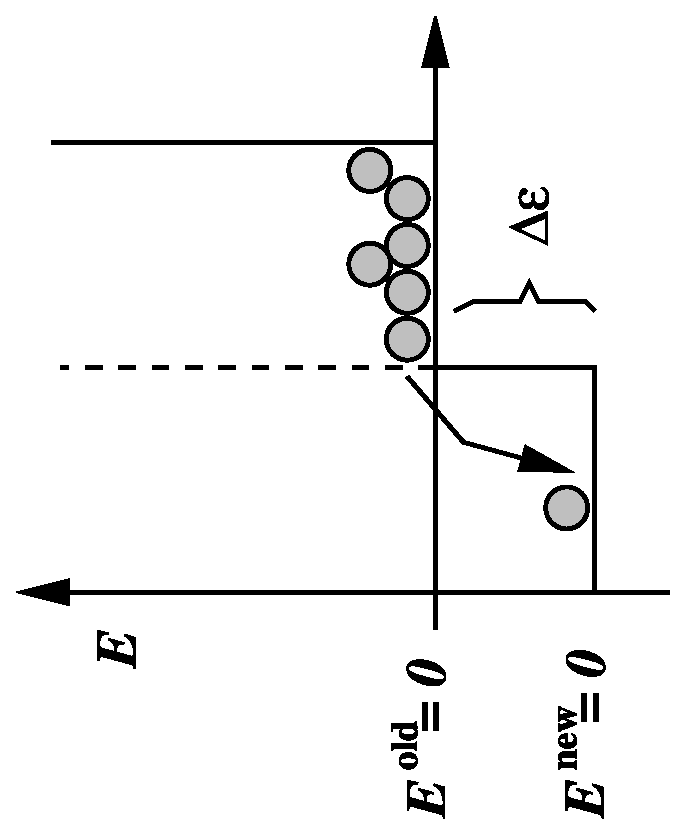
\includegraphics[width=2.1in,angle=-90]{img/fig1.eps}
%\caption{``Energies'' (inferiorities) of strings in a first-order
%  phase transition with latent heat $\Delta\epsilon$.}
%\label{fig1}
%\end{center}
%\end{figure}
